\documentclass{article}
\usepackage[margin=2cm]{geometry}
\usepackage{listings}
\usepackage{float}
\usepackage{graphicx}
\usepackage{natbib}
\usepackage{hyperref}


\lstset{basicstyle=\footnotesize, columns=fullflexible}

\setlength{\parskip}{10pt plus 1pt minus 1pt
\setlength{\parindent}{0cm}}

\begin{document}
\title{CS26410 - Occupancy Grid Mapping Report}
\author{Samuel Jackson \\ \texttt{slj11@aber.ac.uk}}
\date{\today}
\maketitle


\section{Player and Stage}
The Player program together with the Stage plug-in provide a convenient controller and simulator pair used in the field of robotics. Player acts as a wrapper to the hardware specifics of a robot and its sensors and provides an interface for an application to communicate with a physical robot. This is extremely useful, as it allows the developer to easily port code between different types and models of robots with different configurations and sensors without worrying too much about the underlying hardware. It also allows the developer to jump right into developing a robot controller, rather than dealing with code to interface with the system.

The Stage program is a plug-in for Player to create a simulation environment for robotics. Stage takes instructions from the Player application (which in turn is controlled by the developers code) and actuates a model of the robot. In response, Stage also simulates sensor data relative to the position, speed, angle etc. of the robot and feeds it back into Player. This is useful as the development of a robot controller can be built and tested without having access to a physical robot. A simulation program such as Stage allows the core development of robot controllers on a smaller budget and without risk of damaging the robot through unforeseen bugs. The controllers can then be tested, tweaked and improved on a physical robot.

\section{Occupancy Grid Mapping}
Occupancy gird mapping is a robot mapping technique where the world is represented as a discrete number of equally sized, squares called cells. Each of these cells represents a position in a Cartesian coordinate system and can be labelled according to what a robot senses is at this position on the grid (such as if the cell is occupied by an obstacle or not).

\subsection{Representing the world}
In my presented solution, I have split the world into a collection of cells which are 60x60 cm spanning from position (0,0) to an unspecified height and width using a 2D vector representation. Initially, only a grid of 6 x 6 cells are created, but as the robot explores the grid is able to dynamically resize to ensure that the robot never "falls off the map". 

Resizing only occurs when a measured point is found to lay outside of the existing grid. When resizing in a negative direction, we must also shift all data elements forwards/up in order to keep the grid correctly positioned relative to the robot's position.

\begin{center}
	\begin{lstlisting}[language=c++, showstringspaces=false, caption={C++ code for dynamically resizing the grid when a point (x,y) falls outside the current grid's size}]

	if((x < 0 || y < 0) ||(x >= grid_width || y >= grid_height)) {
		
		x_expand = (x < 0 || x >= grid_width) ? EXPANSION_SIZE : 0;
		y_expand = (y < 0 || y >= grid_height) ? EXPANSION_SIZE : 0;

		new_width = grid_width + x_expand;
		new_height = grid_height + y_expand;

		//resize grid to new dimensions
		grid.resize(h);
		for (int i = 0; i < h; ++i) {
 			grid[i].resize(w);
 		}
		
		//if we did a negative resize, shift data
		if(x < 0 || y < 0) {
			robot_x += (x_expand*MAP_SCALE);
			robot_y += (y_expand*MAP_SCALE);

			x += EXPANSION_SIZE;
			y += EXPANSION_SIZE;

			for (int i = (grid_width-1); i >= 0; i--) {
				for (int j = (grid_height-1); j >= 0; j--) {
					int value = GetCell(i,j);
					SetCell(i+x_expand,j+y_expand,value);
					SetCell(i,j,0);
				}
			}
		}

		grid_width = new_width;
		grid_height = new_height;
	}
		
	\end{lstlisting}
\end{center}

Real world values for the robot's change in position are fed into the mapping system and the robot's position in the grid is updated relative to its position in the grid's coordinate system rather than Stage's coordinate system. This is because we require the index of each of cells to be positive so they can be used to index the 2D vector.

\subsection{Sensing the world}
As the robot moves though the environment it can sample data from each of it's sensors and feed the data into the mapping system for evaluation. The sonar sensors used by the Pioneer robots can only give information on the range (between 0-5 metres) of how far away something is relative to the position of the robot.

However, as we know the position of the robot, the angle it's facing and the distance to the sensed object, simple trigonometry can be used to estimate the likely location of the sensed point:

\[ x_{sensed} = x_{robot} + \cos (\theta) \times range \]
\[ y_{sensed} = y_{robot} + \sin (\theta) \times range \]

Where $x_{sensed}$ and $y_{sensed}$ are the position of the sensed point,$x_{robot}$ and $y_{robot}$ are the robot's current position, $\theta$ is the angle the sensor is pointing to and range is the range the sensor measured.

\begin{center}
	\begin{lstlisting}[language=c++, showstringspaces=false, caption={C++ code used for calculating the new point given the current position, angle and range}]

void OccupancyGrid::SensorUpdate(double range, double angle) {
	double sensor_x, sensor_y;

	//offset sensor to side of robot
	range += 0.3;
	
	if (range < MAX_RANGE) {

		//new point hit by sensor
		sensor_x = robot_x + (cos(angle) * range);
		sensor_y = robot_y + (sin(angle) * range);

		//cell index in grid
		grid_x = ScaleToGrid(sensor_x);
		grid_y = ScaleToGrid(sensor_y);

		//calculate degree of certainty that a cell is an obstacle
		double max_grid_r = (MAX_RANGE/MAP_SCALE);
		double range_prob = (max_grid_r-range)/max_grid_r;

		SetCell(grid_x, grid_y, GetCell(grid_x, grid_y) + range_prob);
	}
}

	\end{lstlisting}
\end{center}

Once this new position has been obtained, we can round it to the nearest cell in the grid and mark it as occupied. In my controller, I am adding a value to the cell that represents the certainty we have of the cell being occupied, which is inversely proportional to the range measured. Using this technique we can move through the world, make readings using the robot's sensors and build up a map of the environment.

In my controller, I am using a random wander technique to move through the world. This involves using simple reactive techniques to prevent the Pioneer from crashing into obstacles while still encouraging exploration of the environment. Below I provide a listing of the code I have used to move the robot around the simulated environment and avoiding collisions.

\begin{center}
	\begin{lstlisting}[language=c++, showstringspaces=false, caption={C++ code used to make control the robot to reactively wander through the environment}]

	for (;;) {
		robot.Read();

		//do simple collision avoidance
		if((sp[0] + sp[1]) < (sp[6] + sp[7])) {
			turnrate = dtor(-10);
		} else {
			turnrate = dtor(10);
		}

		if(sp[3] < 0.6 || sp[4] < 0.6) {
			speed = 0;
		} else {
			speed = 0.150;
		}

		//command the motors
		pp.SetSpeed(speed, turnrate);
	}

	\end{lstlisting}
\end{center}

The above system works by trying to keep the robot a balanced distance between the sides using further front sensors. If the distance on one side becomes too small then it turns back towards the other direction. If the distance in front of the robot becomes too small then it reacts by turning on the spot until it has enough room to move forward again. The following screen-shot shows an example output from the terminal once mapping is complete:

\begin{figure}[H]
\centering
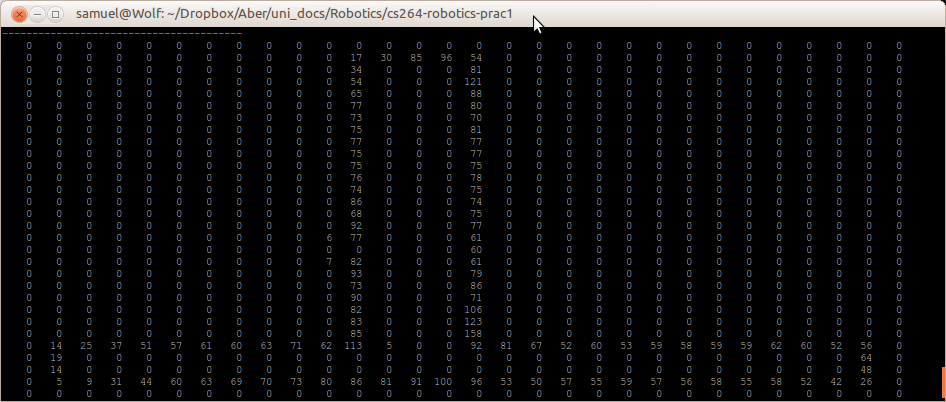
\includegraphics[width=1\textwidth]{example_run.png}
\caption{Console output from a typical simulation.}
\label{fig:example-run}
\end{figure}

\begin{figure}[H]
\centering
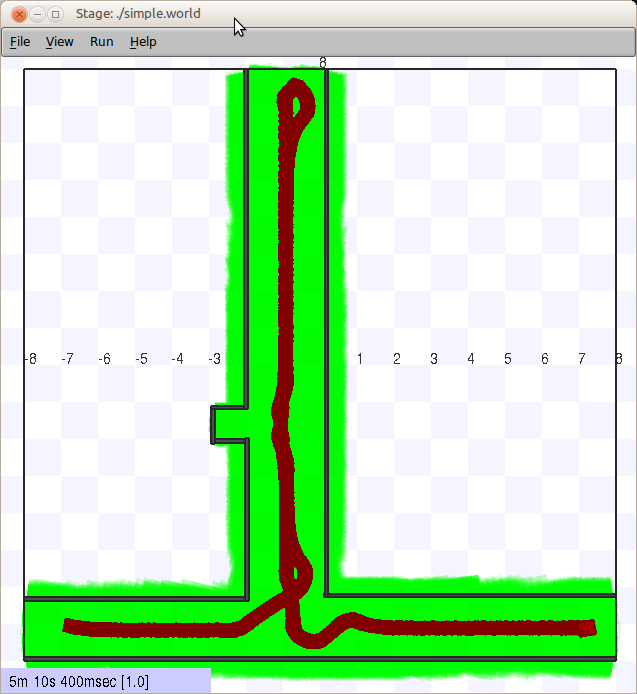
\includegraphics[width=0.7\textwidth]{sim_run.png}
\caption{Path of the robot using random wander.}
\label{fig:example-run}
\end{figure}

\subsection{Interpreting Results}
Once we have mapped the environment, we can begin to analyse the quality of the map and use a threshold to remove any values that appear to be incorrectly identified as obstacles (more on issues with this in section \ref{sec:issues}) The threshold value acts as a cut off point. All values below the threshold are marked as being empty rather than occupied as they have most likely been misidentified. In my application, I have calculated the lower quartile of the data and used this as the threshold. This seemed a reasonable (if somewhat simplistic) choice as it means any cell above 25\% certainty will be classed as an obstacle. 

\begin{center}
	\begin{lstlisting}[language=c++, showstringspaces=false, caption={C++ code used to calculate the threshold value for the grid}]

void OccupancyGrid::CalculateThreshold() {
	using namespace std;
	double average = 0, lower_q = 0;
	vector<double> lq;
	vector<double> vec = VectorUtils::Flatten(grid);
	
	average = VectorUtils::Average(vec);
	vec = VectorUtils::Filter(vec, 0);
	for (int i = 0; i < vec.size(); i++) {
		if(vec[i] <= average) {
			lq.push_back(vec[i]);
		}
	}

	lower_q = VectorUtils::Average(lq);
	cout << "Threshold: " << lower_q+1 << endl;
}

	\end{lstlisting}
\end{center}

The following heat map shows analysis of a typical run of the map. The intensity of colour represents the certainty that the square is a wall. You can see the comparison between the plain map (left) and the map with the threshold applied (right). While this method is by no means perfect, it does help to remove some errors from grid and diminish the presence of others (more on this in section \ref{sec:issues}.
 
\begin{figure}[H]
\centering
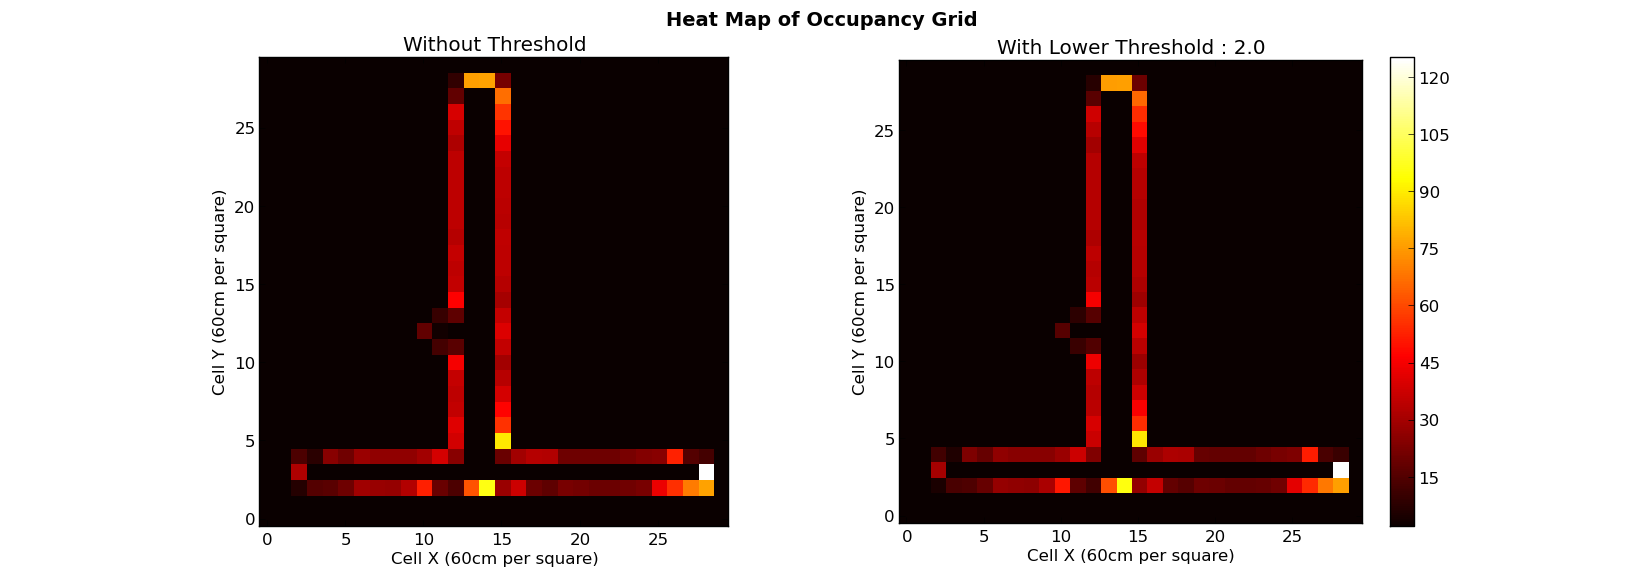
\includegraphics[width=1.1\textwidth]{final_example.png}
\caption{Two Heat Maps showing the certainty that each cell in the grid is a wall, both with and without the threshold. Notice how the incorrect wall cell in the nook is removed in the right hand plot.}
\label{fig:final-example}
\end{figure}

\subsection{Issues and Potential Improvements}
\label{sec:issues}
While I believe I have demonstrated a system that does a reasonable job of mapping an environment, I strongly think that there are several areas of my application that could be vastly improved.

One issue is the inaccuracy of the sensors on the Pioneers and with sonar in general. When a Pioneer senses its environment, it sends out a sonar pulse. This pulse spreads out at an angle of $15\,^\circ$. This means that the actual range measured will not necessarily be at the point exactly calculated from the robot's position, but could be anywhere within this $15\,^\circ$ field of view. Therefore at larger ranges, the accuracy of where the point is becomes less certain. This issue is a major reason why points are incorrectly labelled as walls. Unfortunately, as the only information from the sensor is the range it measured, there is no easy solution to this problem. However there are several ways that it can be diminished. 

One way is to limit the maximum range of a reading so that the pulse does not spread out too much. Another improvement is to only increment a cell by a value that is inversely proportional to the range of the measurement. This means that the value of the cell is directly proportional to the certainty we have about it being a wall. A final improvement that could be made is to use probability based on the contents of surrounding cells (i.e. if all neighbours are walls, this cell is more likely to be a wall). However this approach would prove to be fairly complex and would require a lot more investigation beyond the scope of this report.

Another major issue with occupancy grid mapping is that the world (both simulated and real) cannot always be split into a perfect grid. A wall or obstacle may intersect a cell only partially or at an awkward angle. This means that some space which is actually empty will be marked as being occupied. This problem could be potentially be solved by splitting each cell into a smaller collection of cells and analysing each one using the same technique as before but on a smaller scale. This allows us to achieve a finer degree of accuracy for the reading, but at extra computational overhead. This approach could also be limited by the accuracy that the sensor can read too.

Further improvements could also be made to the threshold value used in mapping. While the current value does a reasonable job of stripping out most of the incorrectly marked cells, it can be affected by outliers with unreasonably high values. It can also be affected if we map the same area more than once, thus giving some cells even double the value. To solve this we could use a clustering technique such as Otsu's method or even K-means in order to find a to separate walls from empty space. However, this technique very much relies on a clear distinction between cells in both categories which may not necessarily be present in the collected data depending on the quality of mapping.

Finally, detection of moving obstacles has not really been considered as part of this report. However I feel that my approach could be developed further to account for moving obstacles. Currently if the robot detects a obstacle the degree of occupancy of a cell is incremented. As more readings hit the obstacle then the degree of occupancy increases and we become more certain that the obstacle exists. If the object disappears while still in range then the occupancy value does not get incremented and therefore, as other cells are marked, will slowly become a less prominent feature in the world until it eventually drops below the threshold and is removed from the map.
\nocite{*}
\bibliographystyle{apalike} % this is one type of author-year style
\bibliography{report_bib.bib}
\end{document}

